% Options for packages loaded elsewhere
\PassOptionsToPackage{unicode}{hyperref}
\PassOptionsToPackage{hyphens}{url}
%
\documentclass[
]{book}
\title{PIPO Project -- WILD6900}
\author{Nadav Mouallem}
\date{2023-03-17}

\usepackage{amsmath,amssymb}
\usepackage{lmodern}
\usepackage{iftex}
\ifPDFTeX
  \usepackage[T1]{fontenc}
  \usepackage[utf8]{inputenc}
  \usepackage{textcomp} % provide euro and other symbols
\else % if luatex or xetex
  \usepackage{unicode-math}
  \defaultfontfeatures{Scale=MatchLowercase}
  \defaultfontfeatures[\rmfamily]{Ligatures=TeX,Scale=1}
\fi
% Use upquote if available, for straight quotes in verbatim environments
\IfFileExists{upquote.sty}{\usepackage{upquote}}{}
\IfFileExists{microtype.sty}{% use microtype if available
  \usepackage[]{microtype}
  \UseMicrotypeSet[protrusion]{basicmath} % disable protrusion for tt fonts
}{}
\makeatletter
\@ifundefined{KOMAClassName}{% if non-KOMA class
  \IfFileExists{parskip.sty}{%
    \usepackage{parskip}
  }{% else
    \setlength{\parindent}{0pt}
    \setlength{\parskip}{6pt plus 2pt minus 1pt}}
}{% if KOMA class
  \KOMAoptions{parskip=half}}
\makeatother
\usepackage{xcolor}
\IfFileExists{xurl.sty}{\usepackage{xurl}}{} % add URL line breaks if available
\IfFileExists{bookmark.sty}{\usepackage{bookmark}}{\usepackage{hyperref}}
\hypersetup{
  pdftitle={PIPO Project -- WILD6900},
  pdfauthor={Nadav Mouallem},
  hidelinks,
  pdfcreator={LaTeX via pandoc}}
\urlstyle{same} % disable monospaced font for URLs
\usepackage{longtable,booktabs,array}
\usepackage{calc} % for calculating minipage widths
% Correct order of tables after \paragraph or \subparagraph
\usepackage{etoolbox}
\makeatletter
\patchcmd\longtable{\par}{\if@noskipsec\mbox{}\fi\par}{}{}
\makeatother
% Allow footnotes in longtable head/foot
\IfFileExists{footnotehyper.sty}{\usepackage{footnotehyper}}{\usepackage{footnote}}
\makesavenoteenv{longtable}
\usepackage{graphicx}
\makeatletter
\def\maxwidth{\ifdim\Gin@nat@width>\linewidth\linewidth\else\Gin@nat@width\fi}
\def\maxheight{\ifdim\Gin@nat@height>\textheight\textheight\else\Gin@nat@height\fi}
\makeatother
% Scale images if necessary, so that they will not overflow the page
% margins by default, and it is still possible to overwrite the defaults
% using explicit options in \includegraphics[width, height, ...]{}
\setkeys{Gin}{width=\maxwidth,height=\maxheight,keepaspectratio}
% Set default figure placement to htbp
\makeatletter
\def\fps@figure{htbp}
\makeatother
\setlength{\emergencystretch}{3em} % prevent overfull lines
\providecommand{\tightlist}{%
  \setlength{\itemsep}{0pt}\setlength{\parskip}{0pt}}
\setcounter{secnumdepth}{5}
\usepackage{booktabs}
\ifLuaTeX
  \usepackage{selnolig}  % disable illegal ligatures
\fi
\usepackage[]{natbib}
\bibliographystyle{plainnat}

\begin{document}
\maketitle

{
\setcounter{tocdepth}{1}
\tableofcontents
}
\hypertarget{about}{%
\chapter{About}\label{about}}

This digital book written in \textbf{Markdown} for Reproducible Data Science (WILD6900).
This book outlines elements of my PIPO project, which studies \emph{pinus ponderosa} (Ponderosa pine, PIPO) regeneration
and plant community composition after high severity reburn wildfires. The content involves the creation of relational
databases in SQL and data visualization with ggplot2 in R.

\hypertarget{database-design-and-structure}{%
\chapter{Database Design and Structure}\label{database-design-and-structure}}

The PIPO project is organized as a relational database, or a collection of related tables.
My project has four interrelated tables:

\begin{enumerate}
\def\labelenumi{\arabic{enumi}.}
\item
  \textbf{PLOTS} : this table has all experimental plots, each with a unique \emph{plot\_id}.
\item
  \textbf{PIPO} : this table has data on ponderosa pine regeneration.
\item
  \textbf{FUELS} : this table has data on fuel loads in each plot, measured in different fuel classes.
\item
  \textbf{COMMUNITY} : this table contains all plant community data, measured as percent cover.
\end{enumerate}

\begin{figure}
\centering
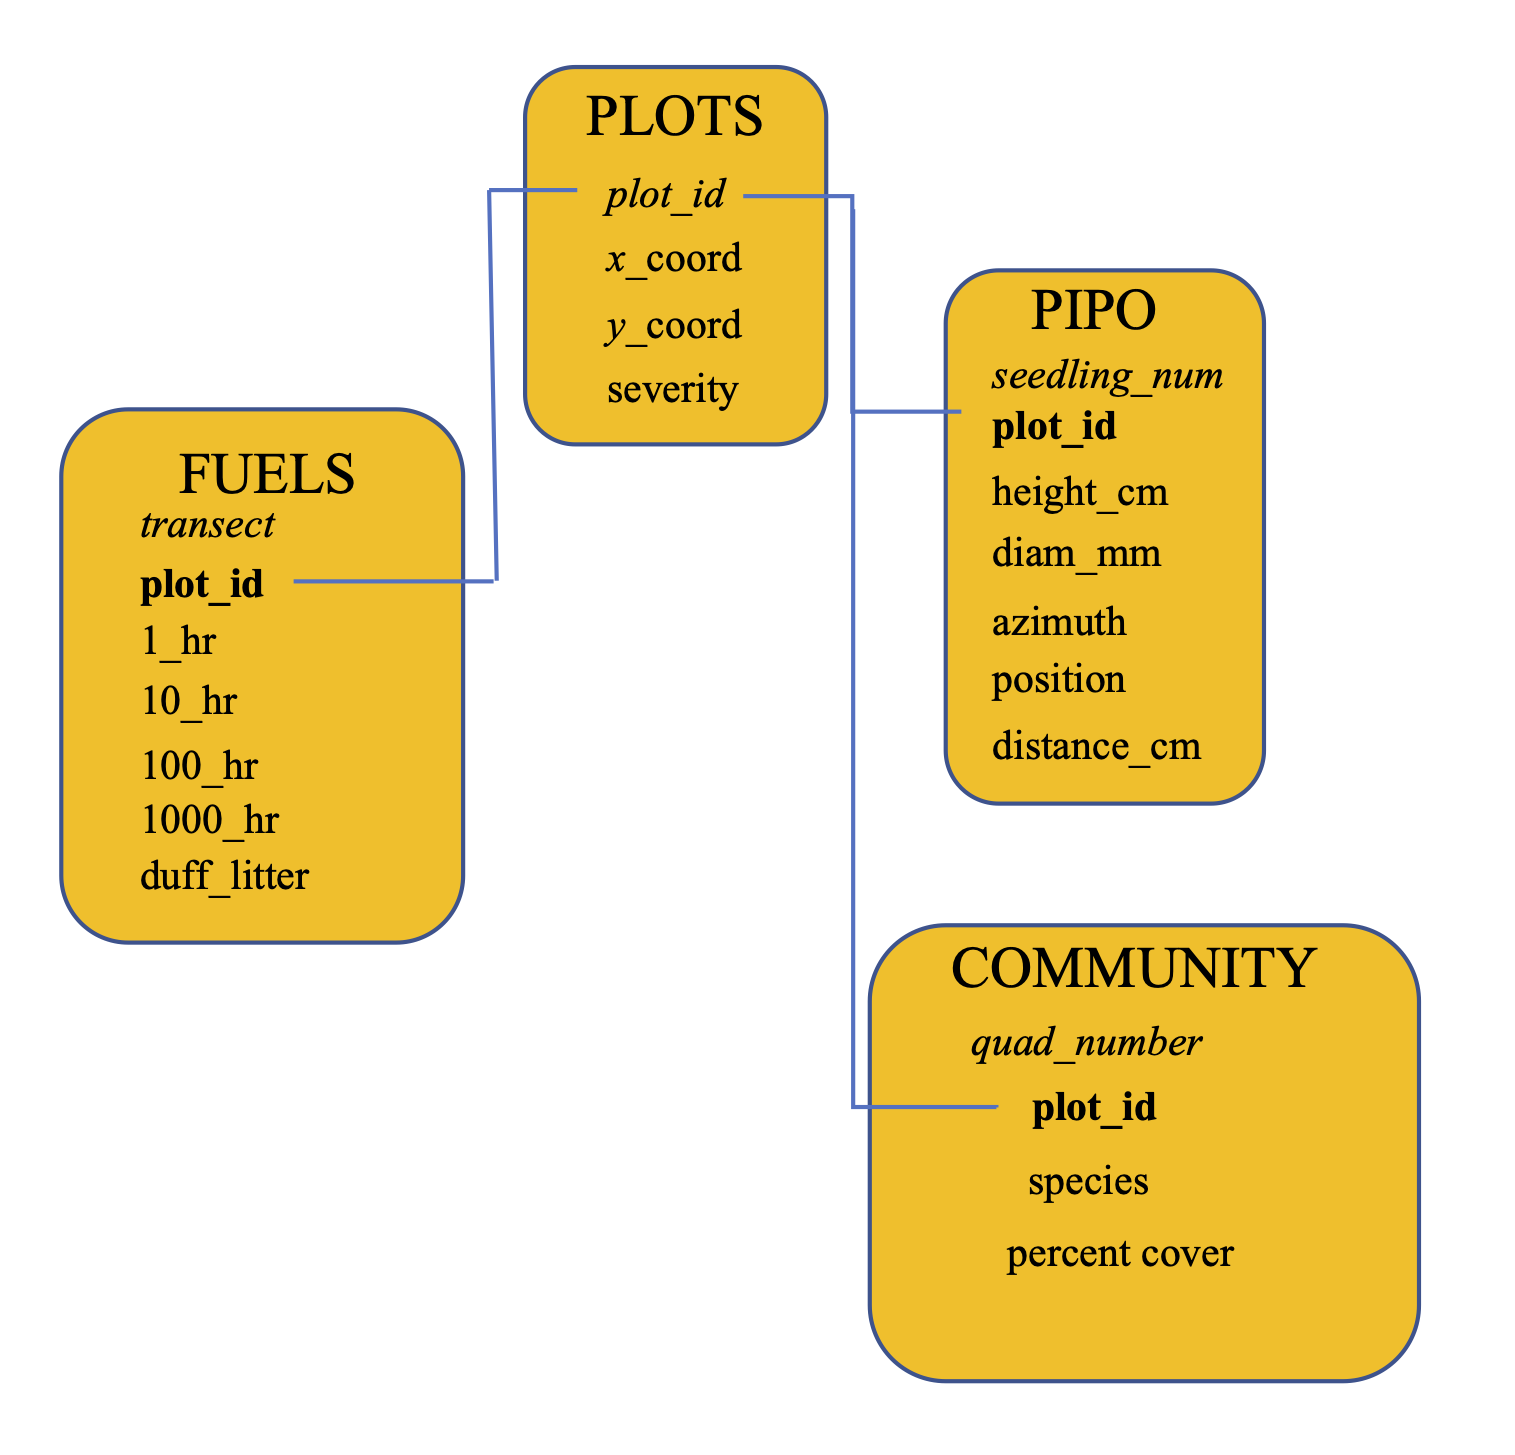
\includegraphics{database_structure_update.png}
\caption{Fig 1. Diagram of the PIPO database.}
\end{figure}

\hypertarget{creating-the-database-structure-in-r}{%
\section{Creating the Database Structure in R}\label{creating-the-database-structure-in-r}}

RSQLite was used in R to create the database in SQL. To start, necessary packages were loaded
and a connection for the database needs to be established.

\begin{verbatim}
# load packages ----
library(DBI)

# establish a connection with the database
PIPO_db <- dbConnect(RSQLite::SQLite(),
                        "/Users/nadav/Documents/USU/Thesis/MS/PIPO.db")
\end{verbatim}

  \bibliography{book.bib,packages.bib}

\end{document}
